\section{Problema de Examen: Varilla Plástica con Camisa Adherida (Alargamientos Parcial 2017)}

\begin{tcolorbox}[colback=white, colframe=myb!80!black, arc=4pt, boxrule=0.9pt, left=8pt, right=8pt, top=7pt, bottom=7pt]
    \textbf{Tipo de Problema:} Barra cilíndrica compuesta con refuerzo coaxial de manguito/camisa adherida (sin deslizamiento relativo en la interfase). Comparación de rigidez axil en tres configuraciones: refuerzo parcial central, refuerzo continuo en toda la longitud y barra simple sin encamisar.\\
    \textbf{Objetivos a Determinar:}
    \begin{enumerate}[label=\alph*)]
        \item \textbf{Alargamiento total de la varilla con camisa central parcial:} Varilla $AD$ de longitud total $L = 0{,}5\text{ m}$ con camisa central de longitud $L_{BC} = 0{,}3\text{ m}$ sometida a axiles de tracción de $P = 15\text{ kN}$.
        \item \textbf{Alargamiento total si la camisa se prolonga a toda la longitud:} Sistema bimetálico/compuesto continuo de $L = 0{,}5\text{ m}$ bajo el mismo axil $P = 15\text{ kN}$.
        \item \textbf{Alargamiento total si no existiera camisa:} Varilla plástica base simple y homogénea de longitud $L = 0{,}5\text{ m}$ bajo $P = 15\text{ kN}$.
    \end{enumerate}
\end{tcolorbox}

\subsection{Enunciado y Propiedades de los Materiales}

Una varilla de plástico maciza de sección circular tiene una longitud total $L = 0{,}5\text{ m} = 500\text{ mm}$ y un diámetro exterior $d_1 = 30\text{ mm}$. Su módulo de elasticidad longitudinal es $E_1 = 3{,}1\text{ GPa} = 3{,}1 \cdot 10^9\text{ N/m}^2$.

Se dispone de una camisa o tubo coaxial del mismo o diferente plástico con longitud $L_2 = 0{,}3\text{ m} = 300\text{ mm}$, diámetro exterior $d_{\text{ext}} = 45\text{ mm}$ y diámetro interior coincidente con el exterior de la varilla ($d_{\text{int}} = d_1 = 30\text{ mm}$). Su módulo elástico es $E_2 = 2{,}5\text{ GPa} = 2{,}5 \cdot 10^9\text{ N/m}^2$.

La camisa está adherida o pegada íntimamente a la varilla en su zona central ($BC$), de forma que \textbf{no existe deslizamiento relativo} entre ambas superficies de contacto (deformación solidaria axil: $\varepsilon_1 = \varepsilon_2$).

\begin{figure}[H]
    \centering
    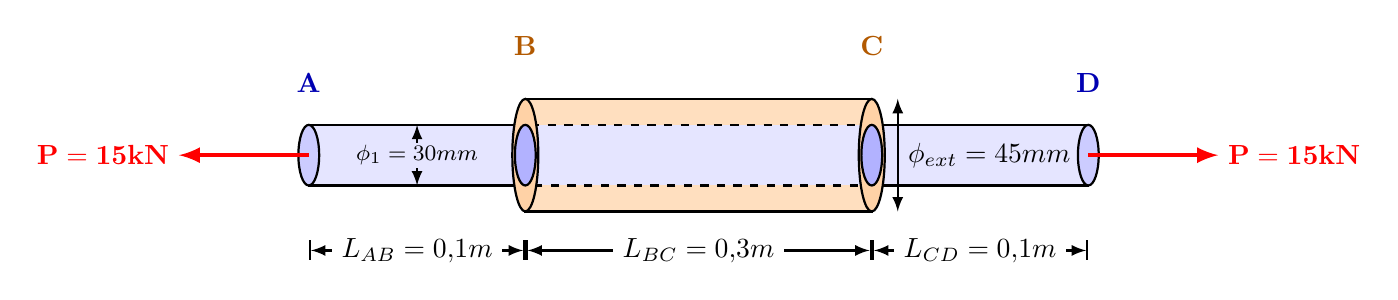
\begin{tikzpicture}[scale=1.1, >=latex]
        % Ejes y líneas de referencia
        % Tramos: A=(0,0), B=(3,0), C=(7.5,0), D=(10.5,0) (escala: 1 unidad = 0.5 dm = 0.05 m)
        % varilla d=30mm -> radio r1=0.35, camisa d=45mm -> radio r2=0.65
        
        % Tramo AB (varilla sola)
        \draw[thick, fill=blue!10] (0,-0.35) rectangle (2.5,0.35);
        
        % Tramo BC (camisa exterior)
        \draw[thick, fill=orange!25] (2.5,-0.65) rectangle (6.5,0.65);
        % Varilla interior (líneas discontinuas dentro de la camisa)
        \draw[dashed, thick, fill=blue!10] (2.5,-0.35) rectangle (6.5,0.35);
        
        % Tramo CD (varilla sola)
        \draw[thick, fill=blue!10] (6.5,-0.35) rectangle (9.0,0.35);
        
        % Tapas circulares / elipses en extremos
        \draw[thick, fill=blue!20] (0,0) ellipse (0.12 and 0.35);
        \draw[thick, fill=orange!35] (2.5,0) ellipse (0.15 and 0.65);
        \draw[thick, fill=blue!30] (2.5,0) ellipse (0.12 and 0.35);
        \draw[thick, fill=orange!35] (6.5,0) ellipse (0.15 and 0.65);
        \draw[thick, fill=blue!30] (6.5,0) ellipse (0.12 and 0.35);
        \draw[thick, fill=blue!20] (9.0,0) ellipse (0.12 and 0.35);
        
        % Cargas de tracción P = 15 kN
        \draw[ultra thick, red, <-] (-1.5,0) -- (0,0);
        \node[red, left] at (-1.5,0) {$\mathbf{P = 15\text{ kN}}$};
        \draw[ultra thick, red, ->] (9.0,0) -- (10.5,0);
        \node[red, right] at (10.5,0) {$\mathbf{P = 15\text{ kN}}$};
        
        % Letras de nudos
        \node[above=8pt, blue!70!black] at (0,0.35) {$\mathbf{A}$};
        \node[above=12pt, orange!70!black] at (2.5,0.65) {$\mathbf{B}$};
        \node[above=12pt, orange!70!black] at (6.5,0.65) {$\mathbf{C}$};
        \node[above=8pt, blue!70!black] at (9.0,0.35) {$\mathbf{D}$};
        
        % Cotas longitudinales
        \draw[|<->|, thick] (0,-1.1) -- (2.5,-1.1) node[midway, fill=white] {$L_{AB} = 0{,}1\text{ m}$};
        \draw[|<->|, thick] (2.5,-1.1) -- (6.5,-1.1) node[midway, fill=white] {$L_{BC} = 0{,}3\text{ m}$};
        \draw[|<->|, thick] (6.5,-1.1) -- (9.0,-1.1) node[midway, fill=white] {$L_{CD} = 0{,}1\text{ m}$};
        
        % Cotas diametrales (reubicadas para no solapar con la carga P = 15 kN)
        \draw[<->, thick] (1.25,-0.35) -- (1.25,0.35) node[midway, fill=blue!10, inner sep=1pt] {\footnotesize $\phi_1 = 30\text{ mm}$};
        \draw[<->, thick] (6.8,-0.65) -- (6.8,0.65) node[midway, right] {$\phi_{\text{ext}} = 45\text{ mm}$};
    \end{tikzpicture}
    \caption{Geometría de la varilla cilíndrica $AD$ con camisa concéntrica pegada en el tramo central $BC$.}
    \label{fig:varilla_camisa_geometria}
\end{figure}

\subsubsection{Cálculo de Áreas y Rigideces Axiles Elementales}

\begin{enumerate}
    \item \textbf{Sección 1 (Varilla maciza de plástico 1):}
    \begin{equation}
        A_1 = \frac{\pi}{4} d_1^2 = \frac{\pi}{4} (0{,}030\text{ m})^2 = \frac{9\pi}{4} \cdot 10^{-4}\text{ m}^2 \approx 7{,}0686 \cdot 10^{-4}\text{ m}^2 = 706{,}86\text{ mm}^2
    \end{equation}
    Rigidez axil unitaria de la varilla:
    \begin{equation}
        (E A)_1 = 3{,}1 \cdot 10^9\text{ N/m}^2 \times 7{,}0686 \cdot 10^{-4}\text{ m}^2 \approx 2{,}1913 \cdot 10^6\text{ N}
    \end{equation}

    \item \textbf{Sección 2 (Camisa tubular de plástico 2):}
    \begin{align}
        A_2 &= \frac{\pi}{4} \left(d_{\text{ext}}^2 - d_1^2\right) = \frac{\pi}{4} \left(0{,}045^2 - 0{,}030^2\right) = \frac{\pi}{4} (0{,}002025 - 0{,}000900) \nonumber \\
        &= \frac{\pi}{4} \cdot 0{,}001125\text{ m}^2 \approx 8{,}8357 \cdot 10^{-4}\text{ m}^2 = 883{,}57\text{ mm}^2
    \end{align}
    Rigidez axil unitaria de la camisa:
    \begin{equation}
        (E A)_2 = 2{,}5 \cdot 10^9\text{ N/m}^2 \times 8{,}8357 \cdot 10^{-4}\text{ m}^2 \approx 2{,}2089 \cdot 10^6\text{ N}
    \end{equation}

    \item \textbf{Rigidez equivalente combinada del tramo compuesto ($BC$):}
    Al estar perfectamente pegadas, ambas secciones experimentan el mismo alargamiento, sumándose sus rigideces:
    \begin{equation}
        (EA)_{\text{eq}} = (EA)_1 + (EA)_2 = 2{,}1913 \cdot 10^6 + 2{,}2089 \cdot 10^6 = 4{,}4002 \cdot 10^6\text{ N}
    \end{equation}
\end{enumerate}

\subsection{Apartado a) Alargamiento Total con Camisa Parcial Central}

El sistema completo está compuesto por tres tramos en serie:
\begin{equation}
    \Delta l_{\text{total}} = \Delta l_{AB} + \Delta l_{BC} + \Delta l_{CD}
\end{equation}

\subsubsection{1. Tramos extremos homogéneos AB y CD (L = 0,1 m)}

En los tramos $AB$ y $CD$, el axil de $15\text{ kN}$ lo soporta íntegramente la varilla maciza:
\begin{equation}
    N_{AB} = N_{CD} = P = 15\text{ kN} = 15\,000\text{ N}
\end{equation}
Aplicando la ley de Hooke unidimensional:
\begin{align}
    \Delta l_{AB} = \Delta l_{CD} &= \frac{P \cdot L_{AB}}{A_1 \cdot E_1} = \frac{15\,000\text{ N} \cdot 0{,}1\text{ m}}{\left(\frac{\pi}{4} \cdot 0{,}03^2\text{ m}^2\right) \cdot \left(3{,}1 \cdot 10^9\text{ N/m}^2\right)} \nonumber \\
    &= \frac{1\,500}{2\,191\,261} \approx 6{,}8454 \cdot 10^{-4}\text{ m} \approx 0{,}6845\text{ mm} \approx 0{,}68\text{ mm}
\end{align}

\subsubsection{2. Tramo central compuesto BC (L = 0,3 m)}

En el tramo $BC$, la carga externa total $P = 15\text{ kN}$ se reparte entre la varilla interna ($N_{BC,1}$) y la camisa externa ($N_{BC,2}$):
\begin{equation}
    N_{BC,1} + N_{BC,2} = P = 15\text{ kN} \label{eq:varilla_camisa_eq_estatica}
\end{equation}

Dado que no existe deslizamiento entre ambas superficies, la deformación axial relativa es nula y los alargamientos de ambos elementos en el tramo coinciden:
\begin{equation}
    \Delta l_{BC,1} = \Delta l_{BC,2} = \Delta l_{BC} \label{eq:varilla_camisa_compatibilidad}
\end{equation}
Sustituyendo por la elasticidad de cada componente:
\begin{equation}
    \frac{N_{BC,1} \cdot L_{BC}}{A_1 \cdot E_1} = \frac{N_{BC,2} \cdot L_{BC}}{A_2 \cdot E_2} \implies N_{BC,1} = N_{BC,2} \frac{A_1 E_1}{A_2 E_2}
\end{equation}
Calculando el cociente de rigideces:
\begin{equation}
    \frac{A_1 E_1}{A_2 E_2} = \frac{7{,}0686 \cdot 10^{-4} \cdot 3{,}1 \cdot 10^9}{8{,}8357 \cdot 10^{-4} \cdot 2{,}5 \cdot 10^9} = \frac{2{,}1913 \cdot 10^6}{2{,}2089 \cdot 10^6} \approx 0{,}9920
\end{equation}
Sustituyendo en la ecuación de equilibrio estático~\eqref{eq:varilla_camisa_eq_estatica}:
\begin{equation}
    0{,}9920\, N_{BC,2} + N_{BC,2} = 15\text{ kN} \implies 1{,}9920\, N_{BC,2} = 15\text{ kN}
\end{equation}
\begin{align}
    N_{BC,2} &= \frac{15}{1{,}9920} \approx \mathbf{7{,}53\text{ kN}} \quad (\text{camisa exterior}) \\
    N_{BC,1} &= 15 - 7{,}53 \approx \mathbf{7{,}47\text{ kN}} \quad (\text{varilla interior})
\end{align}
\begin{tcolorbox}[colback=blue!5!white, colframe=blue!60!black, arc=3pt, boxrule=0.7pt]
    \small \textbf{Comentario sobre la solución manuscrita:}
    En los apuntes de clase se redondeó $A_1 \approx 7{,}1 \cdot 10^{-4}\text{ m}^2$ y $A_2 \approx 8{,}83 \cdot 10^{-4}\text{ m}^2$, obteniéndose valores prácticamente simétricos: $N_{BC,1} = 7{,}49\text{ kN}$ y $N_{BC,2} = 7{,}51\text{ kN}$. Ambos cálculos confirman que la carga de $15\text{ kN}$ se reparte casi al $50\%$ entre varilla y camisa debido a la paridad de sus productos $E \cdot A$.
\end{tcolorbox}

El alargamiento del tramo $BC$ se obtiene evaluando cualquiera de las dos componentes:
\begin{align}
    \Delta l_{BC} &= \frac{N_{BC,1} \cdot L_{BC}}{A_1 \cdot E_1} = \frac{7\,470\text{ N} \cdot 0{,}3\text{ m}}{2{,}1913 \cdot 10^6\text{ N}} \approx 1{,}0229 \cdot 10^{-3}\text{ m} \approx 1{,}02\text{ mm} \approx \mathbf{1{,}00\text{ mm}}
\end{align}
O equivalentemente por la rigidez conjunta:
\begin{equation}
    \Delta l_{BC} = \frac{P \cdot L_{BC}}{(EA)_{\text{eq}}} = \frac{15\,000 \cdot 0{,}3}{4{,}4002 \cdot 10^6} = 1{,}0227 \cdot 10^{-3}\text{ m} \approx 1{,}02\text{ mm}
\end{equation}

\subsubsection{3. Alargamiento total acumulado}

Sumando las deformaciones de los tres tramos:
\begin{align}
    \Delta l_{\text{total, a}} &= \Delta l_{AB} + \Delta l_{BC} + \Delta l_{CD} = 2 \cdot \Delta l_{AB} + \Delta l_{BC} \nonumber \\
    &= 2 \cdot (0{,}6845\text{ mm}) + 1{,}0227\text{ mm} \approx 1{,}369\text{ mm} + 1{,}023\text{ mm} = \mathbf{2{,}39\text{ mm}}
\end{align}
\textit{(En las notas manuscritas redondeadas: $2 \cdot 0{,}68\text{ mm} + 1{,}00\text{ mm} = \mathbf{2{,}36\text{ mm}}$)}.

\subsection{Apartado b) Alargamiento si la Camisa se Prolonga a Toda la Varilla (L = 0,5 m)}

Si la camisa se extiende en la totalidad de la varilla ($L = 0{,}5\text{ m}$), toda la pieza trabaja como una sección compuesta solidaria de longitud completa.

\begin{figure}[H]
    \centering
    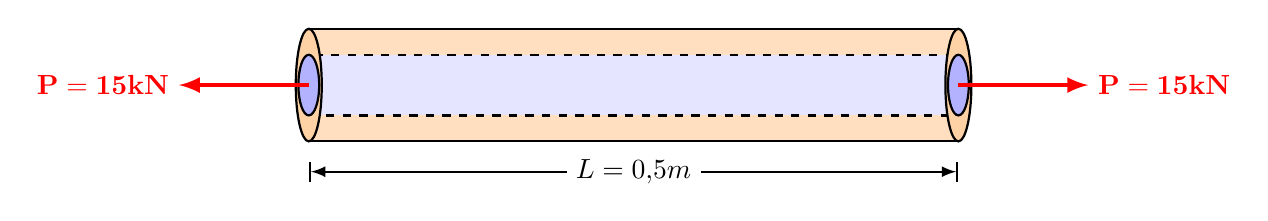
\begin{tikzpicture}[scale=1.1, >=latex]
        % Varilla totalmente encamisada
        \draw[thick, fill=orange!25] (0,-0.65) rectangle (7.5,0.65);
        \draw[dashed, thick, fill=blue!10] (0,-0.35) rectangle (7.5,0.35);
        
        \draw[thick, fill=orange!35] (0,0) ellipse (0.15 and 0.65);
        \draw[thick, fill=blue!30] (0,0) ellipse (0.12 and 0.35);
        \draw[thick, fill=orange!35] (7.5,0) ellipse (0.15 and 0.65);
        \draw[thick, fill=blue!30] (7.5,0) ellipse (0.12 and 0.35);
        
        % Cargas
        \draw[ultra thick, red, <-] (-1.5,0) -- (0,0);
        \node[red, left] at (-1.5,0) {$\mathbf{P = 15\text{ kN}}$};
        \draw[ultra thick, red, ->] (7.5,0) -- (9.0,0);
        \node[red, right] at (9.0,0) {$\mathbf{P = 15\text{ kN}}$};
        
        % Cota longitudinal
        \draw[|<->|, thick] (0,-1.0) -- (7.5,-1.0) node[midway, fill=white] {$L = 0{,}5\text{ m}$};
    \end{tikzpicture}
    \caption{Esquema de la varilla completamente encamisada a lo largo de toda su longitud ($L = 0{,}5\text{ m}$).}
    \label{fig:varilla_camisa_total}
\end{figure}

El reparto de fuerzas entre ambos materiales es idéntico al tramo $BC$ del caso anterior, al mantenerse constantes las propiedades de las secciones y módulos elásticos:
\begin{equation}
    N_1 \approx 7{,}47\text{ kN}, \qquad N_2 \approx 7{,}53\text{ kN}
\end{equation}
El alargamiento total se calcula directamente sobre la longitud total de $0{,}5\text{ m}$:
\begin{equation}
    \Delta l_{\text{total, b}} = \frac{N_1 \cdot L}{A_1 \cdot E_1} = \frac{P \cdot L}{(EA)_{\text{eq}}} = \frac{15\,000\text{ N} \cdot 0{,}5\text{ m}}{4{,}4002 \cdot 10^6\text{ N}} \approx 1{,}704 \cdot 10^{-3}\text{ m} \approx \mathbf{1{,}70\text{ mm}}
\end{equation}
*(Valor redondeado en el manuscrito: $\Delta l = 1{,}7045\text{ mm} \approx \mathbf{1{,}7\text{ mm}}$)*.

\subsection{Apartado c) Alargamiento si No Hubiera Camisa}

En ausencia total de camisa de refuerzo, la varilla maciza de plástico soporta la totalidad del esfuerzo axil $P = 15\text{ kN}$ en toda su longitud $L = 0{,}5\text{ m}$:
\begin{align}
    \Delta l_{\text{total, c}} &= \frac{P \cdot L}{A_1 \cdot E_1} = \frac{15\,000\text{ N} \cdot 0{,}5\text{ m}}{\left(\frac{\pi}{4} \cdot 0{,}03^2\text{ m}^2\right) \cdot \left(3{,}1 \cdot 10^9\text{ N/m}^2\right)} \nonumber \\
    &= \frac{7\,500}{2\,191\,261} \approx 3{,}4226 \cdot 10^{-3}\text{ m} \approx \mathbf{3{,}42\text{ mm}}
\end{align}
*(En el manuscrito se empleó $A_1 \approx 7{,}1 \cdot 10^{-4}\text{ m}^2$, resultando exactamente $\frac{7\,500}{3{,}1 \cdot 10^9 \cdot 7{,}1 \cdot 10^{-4}} \approx 0{,}0034\text{ m} = \mathbf{3{,}4\text{ mm}}$)*.

%=============================================================================
\subsection*{Resumen Comparativo de Configuraciones}

\begin{table}[H]
    \centering
    \caption{Comparación de rigidez y alargamiento de la varilla en función del encamisado ($P = 15\text{ kN}$, $L = 0{,}5\text{ m}$).}
    \vspace{2mm}
    \adjustbox{max width=0.90\textwidth}{%
        \renewcommand{\arraystretch}{1.3}
        \begin{tabular}{lcccc}
            \toprule
            \textbf{Configuración} & \textbf{Rigidez Axil Media} & \textbf{Alargamiento $\Delta l$} & \textbf{Reducción Deformación} & \textbf{Observaciones} \\
            \midrule
            \textbf{c) Sin camisa (solo varilla)} & $(EA)_1 = 2{,}19\text{ MN}$ & $\mathbf{3{,}42\text{ mm}}$ ($3{,}4\text{ mm}$) & $0\%$ (Base) & Varilla de $\phi = 30\text{ mm}$ simple \\
            \textbf{a) Camisa parcial central} & Variable por tramos & $\mathbf{2{,}39\text{ mm}}$ ($2{,}36\text{ mm}$) & $\approx 30{,}1\%$ & Camisa de $0{,}3\text{ m}$ en zona central \\
            \textbf{b) Camisa continua completa} & $(EA)_{\text{eq}} = 4{,}40\text{ MN}$ & $\mathbf{1{,}70\text{ mm}}$ ($1{,}7\text{ mm}$) & $\mathbf{50{,}3\%}$ & Duplica la rigidez axil global \\
            \bottomrule
        \end{tabular}%
    }
    \label{tab:resumen_varilla_camisa}
\end{table}

\begin{tcolorbox}[colback=myg!10!white, colframe=myg!70!black, arc=4pt, boxrule=0.9pt]
    \textbf{Conclusión Física del Problema:}
    \begin{itemize}
        \item En secciones compuestas adheridas en paralelo sometidas a axil directo, la carga total se redistribuye en proporción estricta a la rigidez elástica de cada componente:
        $$\frac{N_1}{N_2} = \frac{E_1 A_1}{E_2 A_2}$$
        \item Al extender la camisa tubular a lo largo de toda la varilla, la rigidez axil prácticamente se duplica ($4{,}40\text{ MN}$ frente a $2{,}19\text{ MN}$), logrando reducir el alargamiento a la mitad exacta ($1{,}70\text{ mm}$ frente a $3{,}42\text{ mm}$).
    \end{itemize}
\end{tcolorbox}

%=============================================================================
\section{Problema de Examen: Columna Rígida con Tirante Inclinado y Carga Lateral}

\begin{tcolorbox}[colback=white, colframe=myb!80!black, arc=4pt, boxrule=0.9pt, left=8pt, right=8pt, top=7pt, bottom=7pt]
    \textbf{Tipo de Problema:} Estructura plana articulada compuesta por una columna vertical indeformable (rígida a flexión) arriostrada mediante un tirante/cable elástico inclinado de acero. Determinación de la capacidad de carga máxima admisible frente a dos estados límite concurrentes: deformabilidad máxima horizontal (flecha o desplazamiento lateral) y resistencia máxima por rotura/tensión admisible en el cable.\\
    \textbf{Objetivos a Determinar:}
    \begin{enumerate}
        \item Carga lateral máxima $P_{\delta}$ admisible para no superar el desplazamiento horizontal admisible del extremo superior $B$: $\delta_{B,h} \leq 11\text{ cm} = 0{,}11\text{ m}$.
        \item Esfuerzo axil máximo $N_{BC,\text{máx}}$ y carga admisible $P_{\sigma}$ para no superar la tensión admisible del cable de acero: $\sigma_{\text{adm}} = 190\text{ N/mm}^2 = 190\text{ MPa}$.
        \item Carga máxima admisible de servicio global del sistema: $P_{\text{máx}} = \min(P_{\delta}, P_{\sigma})$.
    \end{enumerate}
\end{tcolorbox}

\subsection{Enunciado y Geometría de Partida}

Se considera la estructura mostrada en la figura, formada por una columna vertical $AB$ considerada infinitamente rígida e indeformable, articulada en su base $A$ mediante un apoyo fijo. La altura total de la columna es:
\begin{equation}
    H = L_{AB} = 3{,}5\text{ m} + 2{,}5\text{ m} = 6{,}0\text{ m}
\end{equation}
Sobre la columna actúa una carga horizontal puntual $P$ hacia la izquierda, aplicada a una cota de $3{,}5\text{ m}$ sobre la base ($2{,}5\text{ m}$ por debajo del extremo superior $B$).

Para impedir el vuelco y restringir el desplazamiento lateral de la columna, se ancla en su cúspide $B$ un cable elástico de acero $BC$, que se fija a tierra en un punto rígido $C$ situado al nivel del suelo a una distancia horizontal de $4{,}0\text{ m}$ respecto al eje de la columna. El anclaje $C$ es un punto de apoyo fijo independiente.

\begin{figure}[H]
    \centering
    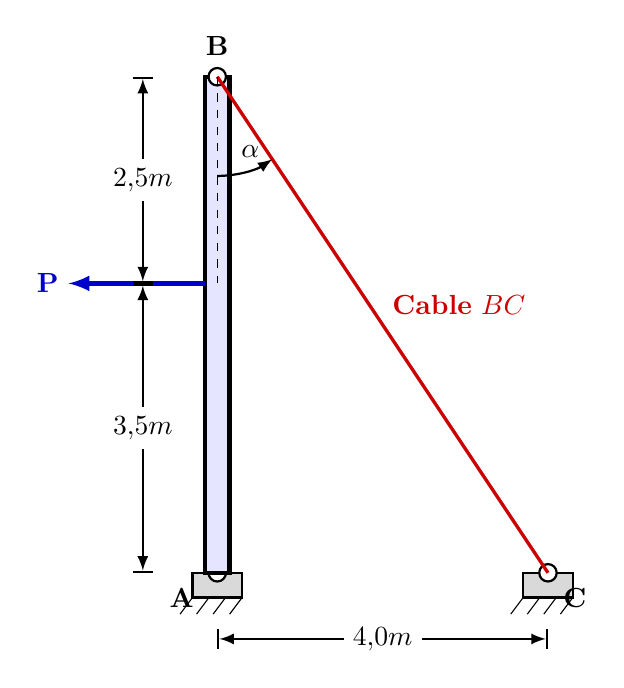
\begin{tikzpicture}[scale=1.05, >=latex]
        % Apoyo A en (0,0)
        \draw[thick, fill=gray!30] (-0.3,-0.3) rectangle (0.3,0);
        \draw (-0.3,-0.3) -- (-0.45,-0.5);
        \draw (-0.1,-0.3) -- (-0.25,-0.5);
        \draw (0.1,-0.3) -- (-0.05,-0.5);
        \draw (0.3,-0.3) -- (0.15,-0.5);
        \draw[thick, fill=white] (0,0) circle (3pt);
        \node[below left=2pt] at (-0.1,0) {$\mathbf{A}$};
        
        % Barra vertical rígida AB
        \draw[ultra thick, fill=blue!10] (-0.15,0) rectangle (0.15,6.0);
        \draw[thick, fill=white] (0,6.0) circle (3pt);
        \node[above=4pt] at (0,6.0) {$\mathbf{B}$};
        
        % Anclaje C en (4.0, 0)
        \draw[thick, fill=gray!30] (3.7,-0.3) rectangle (4.3,0);
        \draw (3.7,-0.3) -- (3.55,-0.5);
        \draw (3.9,-0.3) -- (3.75,-0.5);
        \draw (4.1,-0.3) -- (3.95,-0.5);
        \draw (4.3,-0.3) -- (4.15,-0.5);
        \draw[thick, fill=white] (4.0,0) circle (3pt);
        \node[below right=2pt] at (4.0,0) {$\mathbf{C}$};
        
        % Cable BC
        \draw[very thick, red!80!black] (0,6.0) -- (4.0,0);
        \node[red!80!black, above right] at (2.0,3.0) {\textbf{Cable} $BC$};
        
        % Carga horizontal P en y = 3.5m
        \draw[ultra thick, blue!80!black, <-] (-1.8,3.5) -- (-0.15,3.5);
        \node[blue!80!black, left] at (-1.8,3.5) {$\mathbf{P}$};
        
        % Ángulo alfa en B
        \draw[dashed, thin] (0,6.0) -- (0,3.5);
        \draw[thick, ->] (0,4.8) arc (-90:-56.3:1.2);
        \node at (0.4,5.1) {$\alpha$};
        
        % Cotas verticales
        \draw[|<->|, thick] (-0.9,0) -- (-0.9,3.5) node[midway, fill=white] {$3{,}5\text{ m}$};
        \draw[|<->|, thick] (-0.9,3.5) -- (-0.9,6.0) node[midway, fill=white] {$2{,}5\text{ m}$};
        
        % Cota horizontal
        \draw[|<->|, thick] (0,-0.8) -- (4.0,-0.8) node[midway, fill=white] {$4{,}0\text{ m}$};
    \end{tikzpicture}
    \caption{Geometría de la columna rígida $AB$ arriostrada mediante el cable inclinado $BC$.}
    \label{fig:columna_tirante_geometria}
\end{figure}

\subsubsection{Propiedades Mecánicas y Geométricas del Cable}

\begin{itemize}
    \item \textbf{Diámetro nominal del cable:} $\phi = 4\text{ mm} = 4 \cdot 10^{-3}\text{ m}$.
    \item \textbf{Sección transversal del cable ($\Omega$):}
    \begin{equation}
        \Omega = \frac{\pi}{4}\phi^2 = \frac{\pi}{4}(4 \cdot 10^{-3}\text{ m})^2 = 4\pi \cdot 10^{-6}\text{ m}^2 \approx 1{,}2566 \cdot 10^{-5}\text{ m}^2 = 12{,}566\text{ mm}^2
    \end{equation}
    \item \textbf{Módulo de elasticidad longitudinal ($E$):}
    \begin{equation}
        E = 20\,000\text{ kN/cm}^2 = 20\,000 \cdot \frac{10^3\text{ N}}{10^{-4}\text{ m}^2} = 2 \cdot 10^{11}\text{ N/m}^2 = 200\text{ GPa}
    \end{equation}
    \item \textbf{Tensión admisible de rotura/servicio ($\sigma_{\text{adm}}$):}
    \begin{equation}
        \sigma_{\text{adm}} = 190\text{ N/mm}^2 = 190\text{ MPa} = 190 \cdot 10^6\text{ N/m}^2
    \end{equation}
    \item \textbf{Desplazamiento horizontal máximo admisible de la cúspide $B$:}
    \begin{equation}
        \delta_{B,h} = \overline{BB''} \leq 11\text{ cm} = 0{,}11\text{ m}
    \end{equation}
    \item \textbf{Longitud y orientación geométrica del cable $BC$:}
    \begin{align}
        L_C &= \sqrt{4{,}0^2 + 6{,}0^2} = \sqrt{16 + 36} = \sqrt{52}\text{ m} \approx 7{,}2111\text{ m} \approx 7{,}21\text{ m} \\
        \tan \alpha &= \frac{4{,}0}{6{,}0} = \frac{2}{3} \implies \alpha = \arctan\left(\frac{2}{3}\right) \approx 33{,}69^\circ \\
        \sin \alpha &= \frac{4}{\sqrt{52}} = \frac{2}{\sqrt{13}} \approx 0{,}5547 \\
        \cos \alpha &= \frac{6}{\sqrt{52}} = \frac{3}{\sqrt{13}} \approx 0{,}8321
    \end{align}
\end{itemize}

\subsection{Equilibrio Estático de la Columna Rígida}

Aislando la columna rígida $AB$, las fuerzas que intervienen en su Diagrama de Sólido Libre (DCL) son:
\begin{enumerate}
    \item Reacciones en el apoyo fijo $A$: componente horizontal $H_A$ ($\rightarrow$) y componente vertical $V_A$ ($\uparrow$).
    \item Carga horizontal exterior aplicada $P$ ($\leftarrow$) a cota $y = 3{,}5\text{ m}$.
    \item Acción del cable $BC$ sobre la cúspide $B$: fuerza de tracción $N_{BC}$ dirigida a lo largo del cable hacia el anclaje $C$, cuyas componentes son:
    \begin{align}
        N_{BC,x} &= N_{BC} \sin\alpha \quad (\rightarrow) \\
        N_{BC,y} &= N_{BC} \cos\alpha \quad (\downarrow)
    \end{align}
\end{enumerate}

\begin{figure}[H]
    \centering
    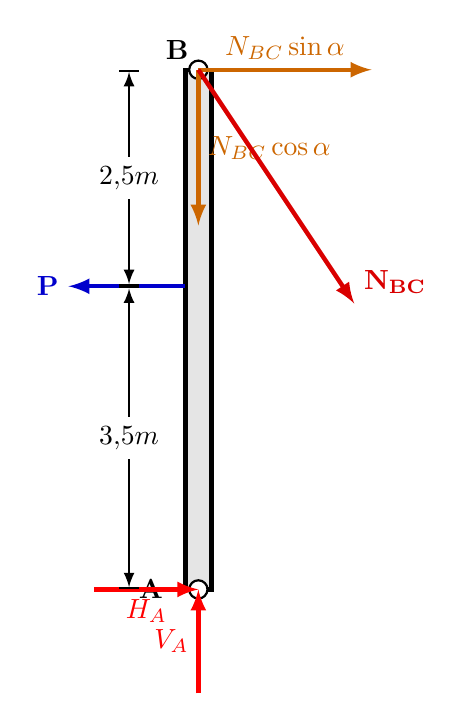
\begin{tikzpicture}[scale=1.1, >=latex]
        % Columna
        \draw[ultra thick, fill=gray!20] (-0.15,0) rectangle (0.15,6.0);
        
        % Apoyo A
        \draw[thick, fill=white] (0,0) circle (3pt);
        \node[left=3pt] at (-0.2,0) {$\mathbf{A}$};
        \draw[ultra thick, red, ->] (-1.2,0) -- (0,0);
        \node[red, below] at (-0.6,0) {$H_A$};
        \draw[ultra thick, red, ->] (0,-1.2) -- (0,0);
        \node[red, left] at (0,-0.6) {$V_A$};
        
        % Carga P
        \draw[ultra thick, blue!80!black, <-] (-1.5,3.5) -- (-0.15,3.5);
        \node[blue!80!black, left] at (-1.5,3.5) {$\mathbf{P}$};
        
        % Descomposición de la fuerza en B
        \draw[thick, fill=white] (0,6.0) circle (3pt);
        \node[above left] at (0,6.0) {$\mathbf{B}$};
        \draw[ultra thick, orange!80!black, ->] (0,6.0) -- (2.0,6.0);
        \node[orange!80!black, above] at (1.0,6.0) {$N_{BC} \sin\alpha$};
        \draw[ultra thick, orange!80!black, ->] (0,6.0) -- (0,4.2);
        \node[orange!80!black, right] at (0,5.1) {$N_{BC} \cos\alpha$};
        \draw[ultra thick, red!85!black, ->] (0,6.0) -- (1.8,3.3);
        \node[red!85!black, above right] at (1.8,3.3) {$\mathbf{N_{BC}}$};
        
        % Cotas
        \draw[|<->|, thick] (-0.8,0) -- (-0.8,3.5) node[midway, fill=white] {$3{,}5\text{ m}$};
        \draw[|<->|, thick] (-0.8,3.5) -- (-0.8,6.0) node[midway, fill=white] {$2{,}5\text{ m}$};
    \end{tikzpicture}
    \caption{Diagrama de Sólido Libre (DCL) de la columna rígida $AB$.}
    \label{fig:columna_dcl}
\end{figure}

Planteando las tres ecuaciones de equilibrio estático en el plano:
\begin{align}
    \sum F_x = 0 &\implies H_A - P + N_{BC} \sin\alpha = 0 \label{eq:columna_fx} \\
    \sum F_y = 0 &\implies V_A - N_{BC} \cos\alpha = 0 \label{eq:columna_fy} \\
    \sum M_A = 0 &\implies P \cdot 3{,}5 - (N_{BC} \sin\alpha) \cdot 6{,}0 = 0 \label{eq:columna_ma}
\end{align}

De la ecuación de momentos~\eqref{eq:columna_ma} se obtiene la relación directa e independiente entre la fuerza del tirante $N_{BC}$ y la carga lateral $P$:
\begin{equation}
    P \cdot 3{,}5 = N_{BC} \cdot 6{,}0 \cdot \sin(33{,}69^\circ) = N_{BC} \cdot 6{,}0 \cdot \frac{2}{\sqrt{13}} \approx 3{,}3282 \, N_{BC}
\end{equation}
\begin{equation}
    P = \frac{6{,}0 \cdot \sin(33{,}69^\circ)}{3{,}5} N_{BC} \approx 0{,}9509 \, N_{BC} \label{eq:relacion_p_nbc}
\end{equation}

\subsection{Análisis Cinemático y Condición de Compatibilidad}

Al ser la barra $AB$ rígida e indeformable articulada en $A$, su deformada corresponde a una rotación pura de sólido rígido alrededor de $A$ por un ángulo infinitesimal $\theta$.
El extremo $B$ sufre un desplazamiento horizontal:
\begin{equation}
    \delta_{B,h} = \overline{BB''} = H \cdot \theta \leq 0{,}11\text{ m}
\end{equation}

\begin{figure}[H]
    \centering
    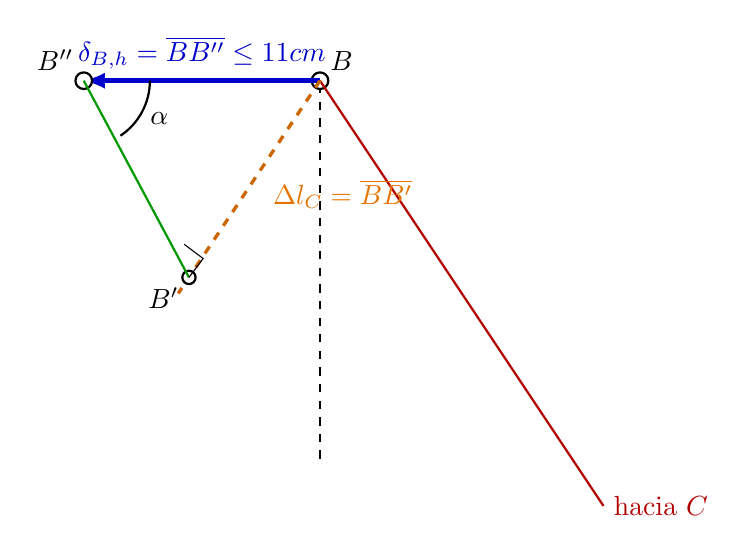
\begin{tikzpicture}[scale=1.2, >=latex]
        % Triángulo cinemático en el nudo B
        \coordinate (B) at (0,4);
        \coordinate (Bpp) at (-2.5,4); % Desplazamiento horizontal B''
        \coordinate (Bp) at (-1.387,1.919); % Proyección sobre la dirección del cable
        
        % Línea original de la barra
        \draw[thick, dashed] (0,0) -- (B);
        \draw[thick, fill=white] (B) circle (2.5pt) node[above right] {$B$};
        
        % Cable original hacia C
        \draw[thick, red!70!black] (B) -- (3, -0.5) node[right] {hacia $C$};
        
        % Desplazamiento horizontal BB''
        \draw[ultra thick, blue!80!black, ->] (B) -- (Bpp) node[midway, above] {$\delta_{B,h} = \overline{BB''} \leq 11\text{ cm}$};
        \draw[thick, fill=white] (Bpp) circle (2.5pt) node[above left] {$B''$};
        
        % Alargamiento del cable Delta l_C = BB'
        \draw[very thick, dashed, orange!80!black] (B) -- (-1.5,1.75);
        \draw[thick, fill=white] (-1.387,1.919) circle (2pt) node[below left] {$B'$};
        
        % Triángulo rectángulo B - B' - B''
        \draw[thick, green!60!black] (Bpp) -- (-1.387,1.919);
        
        % Ángulo recto en B'
        \draw[thin] (-1.387,1.919) -- ++(0.15,0.2) -- ++(-0.2,0.15);
        
        % Cota de alargamiento Delta l
        \node[orange!90!black, right] at (-0.6,2.8) {$\Delta l_C = \overline{BB'}$};
        
        % Ángulo alfa
        \draw[thick] (Bpp) ++(0.7,0) arc (0:-56.3:0.7);
        \node at (-1.7,3.6) {$\alpha$};
    \end{tikzpicture}
    \caption{Cinemática del nudo $B$: proyección geométrica del desplazamiento lateral $\delta_{B,h}$ en el alargamiento axial del cable $\Delta l_C$.}
    \label{fig:cinematica_cable}
\end{figure}

Proyectando el desplazamiento horizontal $\delta_{B,h} = \overline{BB''}$ sobre la directriz del cable inclinado (formando el triángulo rectángulo $BB'B''$ con ángulo recto en $B'$):
\begin{equation}
    \sin\alpha = \frac{\Delta l_C}{\overline{BB''}} \implies \Delta l_C = \overline{BB''} \cdot \sin\alpha \label{eq:compatibilidad_cable}
\end{equation}

Sustituyendo el desplazamiento horizontal admisible $\overline{BB''} \leq 0{,}11\text{ m}$:
\begin{equation}
    \Delta l_{C,\text{máx}} = 0{,}11\text{ m} \cdot \sin(33{,}69^\circ) = 0{,}11 \cdot 0{,}5547 \approx 0{,}0610\text{ m} = 61{,}0\text{ mm}
\end{equation}

\subsection{Cálculo de la Capacidad de Carga Frente a Cada Estado Límite}

\subsubsection{1. Limitación por Deformabilidad (Flecha máxima admisible)}

Relacionando el alargamiento elástico del cable con su ley constitutiva (Hooke):
\begin{equation}
    \Delta l_C = \frac{N_{BC} \cdot L_C}{\Omega \cdot E} \implies N_{BC,\delta} = \frac{\Delta l_{C,\text{máx}} \cdot \Omega \cdot E}{L_C}
\end{equation}
Sustituyendo los valores numéricos del sistema:
\begin{align}
    N_{BC,\delta} &= \frac{0{,}0610\text{ m} \cdot \left(1{,}2566 \cdot 10^{-5}\text{ m}^2\right) \cdot \left(2 \cdot 10^{11}\text{ N/m}^2\right)}{7{,}2111\text{ m}} \nonumber \\
    &= \frac{153\,305{,}2}{7{,}2111} \approx 21\,259{,}6\text{ N} \approx \mathbf{21{,}26\text{ kN}}
\end{align}
A partir del equilibrio de momentos~\eqref{eq:columna_ma}, la carga exterior $P$ asociada a este límite de deformación es:
\begin{equation}
    P_{\delta} = \frac{6{,}0 \cdot \sin(33{,}69^\circ)}{3{,}5} \cdot 21{,}26\text{ kN} \approx \mathbf{20{,}21\text{ kN}}
\end{equation}

\subsubsection{2. Comprobación y Limitación por Tensión Admisible}

Si se aplicara la carga calculada por deformación ($N_{BC} = 21{,}26\text{ kN}$), la tensión de trabajo efectiva en el cable resultaría:
\begin{equation}
    \sigma = \frac{N_{BC,\delta}}{\Omega} = \frac{21\,260\text{ N}}{12{,}566\text{ mm}^2} \approx 1\,691{,}9\text{ N/mm}^2 \approx \mathbf{1692\text{ MPa}} \gg \sigma_{\text{adm}} = 190\text{ MPa}
\end{equation}
\begin{tcolorbox}[colback=red!10!white, colframe=red!80!black, arc=3pt, boxrule=0.9pt]
    \textbf{¡Aviso de Inadmisibilidad!:}\\
    La tensión de $1692\text{ MPa}$ supera en casi 9 veces la tensión admisible del acero ($\sigma_{\text{adm}} = 190\text{ MPa}$). Por tanto, \textbf{el cable rompería plásticamente mucho antes} de alcanzar el desplazamiento horizontal de $11\text{ cm}$. La resistencia del cable es el estado límite crítico determinante.
\end{tcolorbox}

Por consiguiente, el esfuerzo axil máximo admisible que el cable de $4\text{ mm}$ puede soportar con seguridad es:
\begin{align}
    N_{BC,\text{adm}} &= \sigma_{\text{adm}} \cdot \Omega = 190\text{ N/mm}^2 \times 12{,}566\text{ mm}^2 \nonumber \\
    &= 2\,387{,}54\text{ N} \approx \mathbf{2{,}39\text{ kN}}
\end{align}

Sustituyendo este esfuerzo axil en la ecuación de momentos~\eqref{eq:columna_ma}:
\begin{equation}
    P_{\sigma} = \frac{6{,}0 \cdot \sin(33{,}69^\circ)}{3{,}5} \cdot 2{,}3875\text{ kN} = 0{,}9509 \cdot 2{,}3875\text{ kN} \approx \mathbf{2{,}27\text{ kN}}
\end{equation}

\subsubsection{3. Desplazamiento Real en Régimen Admisible}

Bajo la carga admisible real de $P = 2{,}27\text{ kN}$, el alargamiento y el desplazamiento horizontal en $B$ resultan:
\begin{align}
    \Delta l_C &= \frac{N_{BC,\text{adm}} \cdot L_C}{\Omega \cdot E} = \frac{\sigma_{\text{adm}} \cdot L_C}{E} = \frac{190 \cdot 10^6\text{ N/m}^2 \cdot 7{,}2111\text{ m}}{2 \cdot 10^{11}\text{ N/m}^2} \approx 6{,}85\text{ mm} \\
    \delta_{B,h} &= \frac{\Delta l_C}{\sin\alpha} = \frac{6{,}85\text{ mm}}{\sin(33{,}69^\circ)} \approx \mathbf{12{,}35\text{ mm}} = 1{,}24\text{ cm} \ll 11\text{ cm}
\end{align}

\subsection{Cálculo de Reacciones en la Base A}

Bajo la carga de servicio máxima admisible $P_{\text{máx}} = 2{,}27\text{ kN}$ ($N_{BC} = 2{,}39\text{ kN}$):
\begin{align}
    H_A &= P - N_{BC}\sin\alpha = 2{,}27\text{ kN} - 2{,}39 \cdot 0{,}5547\text{ kN} \approx 2{,}27 - 1{,}33 = \mathbf{0{,}94\text{ kN}} \quad (\rightarrow) \\
    V_A &= N_{BC}\cos\alpha = 2{,}39 \cdot 0{,}8321\text{ kN} \approx \mathbf{1{,}99\text{ kN}} \quad (\uparrow)
\end{align}

%=============================================================================
\subsection*{Resumen Final de Resultados}

\begin{table}[H]
    \centering
    \caption{Comparación de estados límites y dimensionamiento de la carga admisible $P$.}
    \vspace{2mm}
    \adjustbox{max width=0.98\textwidth}{%
        \renewcommand{\arraystretch}{1.25}
        \begin{tabular}{lccc}
            \toprule
            \textbf{Criterio / Condición} & \textbf{Esfuerzo Cable $N_{BC}$} & \textbf{Carga Lateral $P$} & \textbf{Estado / Diagnóstico} \\
            \midrule
            \textbf{1. Deformabilidad ($\delta_B \leq 11\text{ cm}$)} & $21{,}26\text{ kN}$ & $20{,}21\text{ kN}$ & Inadmisible ($\sigma = 1692\text{ MPa} \gg \sigma_{\text{adm}}$) \\
            \textbf{2. Tensión Admisible ($\sigma \leq 190\text{ MPa}$)} & $\mathbf{2{,}39\text{ kN}}$ & $\mathbf{2{,}27\text{ kN}}$ & \textbf{Límite Determinante (Válido)} \\
            \midrule
            \multicolumn{4}{l}{\textbf{Respuesta Final:} $\mathbf{P_{\text{máx}} = 2{,}27\text{ kN}}$ (Desplazamiento horizontal resultante: $\delta_B = 1{,}24\text{ cm} \leq 11\text{ cm}$)} \\
            \bottomrule
        \end{tabular}%
    }
    \label{tab:resumen_columna_tirante}
\end{table}

\begin{tcolorbox}[colback=myg!10!white, colframe=myg!70!black, arc=4pt, boxrule=0.9pt]
    \textbf{Nota Conceptual del Problema:}
    \begin{itemize}
        \item Cuando en un problema de resistencia de materiales se imponen simultáneamente condiciones de \textbf{deformabilidad máxima} (rigidez/flecha) y de \textbf{tensión admisible} (resistencia), la capacidad de carga real de la estructura viene estrictamente fijada por el mínimo de ambas:
        $$P_{\text{máx}} = \min(P_{\delta}, P_{\sigma})$$
        \item En este caso, el cable de $\phi = 4\text{ mm}$ es muy esbelto, por lo que alcanza su límite resistente con una deformación elástica moderada ($1{,}24\text{ cm}$), quedando la restricción geométrica de $11\text{ cm}$ con un amplio margen de seguridad.
    \end{itemize}
\end{tcolorbox}

%=============================================================================
\section{Problema de Examen: Barra Escalonada Biapoyada Bajo Peso Propio (Febrero 2016)}

\begin{tcolorbox}[colback=white, colframe=myb!80!black, arc=4pt, boxrule=0.9pt, left=8pt, right=8pt, top=7pt, bottom=7pt]
    \textbf{Tipo de Problema:} Barra vertical escalonada de dos tramos de diferente sección transversal, coaccionada axialmente en ambos extremos (biapoyada / biempotrada axil) y solicitada exclusivamente por su \textbf{peso propio continuo}.\\
    \textbf{Objetivos a Determinar:}
    \begin{enumerate}[label=\alph*)]
        \item Reacciones en los apoyos extremos ($R_A$ y $R_C$).
        \item Ley analítica y diagramas de esfuerzos axiles $N(x)$ y tensiones normales $\sigma(x)$ a lo largo de toda la barra $ABC$.
    \end{enumerate}
\end{tcolorbox}

\subsection{Enunciado y Geometría de Partida}

Se considera una barra vertical de directriz recta escalonada en dos tramos, anclada en sus extremos superior $A$ e inferior $C$ mediante apoyos rígidos que impiden todo desplazamiento vertical ($\Delta L_{AC} = 0$).

\begin{figure}[H]
    \centering
    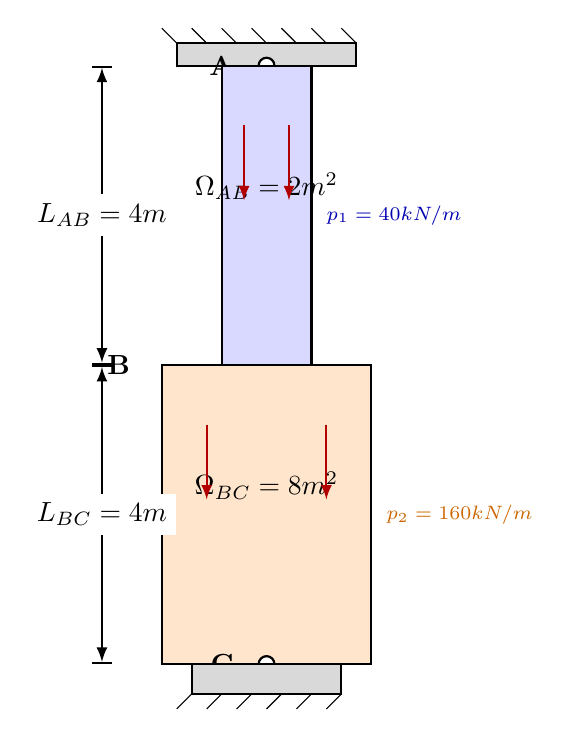
\begin{tikzpicture}[scale=0.95, >=latex]
        % Apoyo superior A
        \draw[thick, fill=gray!30] (-1.2,8) rectangle (1.2,8.3);
        \draw (-1.2,8.3) -- (-1.4,8.5);
        \draw (-0.8,8.3) -- (-1.0,8.5);
        \draw (-0.4,8.3) -- (-0.6,8.5);
        \draw (0.0,8.3) -- (-0.2,8.5);
        \draw (0.4,8.3) -- (0.2,8.5);
        \draw (0.8,8.3) -- (0.6,8.5);
        \draw (1.2,8.3) -- (1.0,8.5);
        \draw[thick, fill=white] (0,8) circle (3pt);
        \node[left=3pt] at (-0.2,8) {$\mathbf{A}$};
        
        % Tramo superior AB (Sección menor Omega_1 = 2 m^2)
        \draw[thick, fill=blue!15] (-0.6,4) rectangle (0.6,8);
        \node[above=2pt] at (0,6) {$\Omega_{AB} = 2\text{ m}^2$};
        \node[right=2pt, font=\scriptsize, blue!70!black] at (0.6,6) {$p_1 = 40\text{ kN/m}$};
        
        % Flechas de peso propio en AB
        \draw[thick, red!70!black, ->] (-0.3,7.2) -- (-0.3,6.2);
        \draw[thick, red!70!black, ->] (0.3,7.2) -- (0.3,6.2);
        
        % Nudo intermedio B
        \node[left=8pt] at (-1.4,4) {$\mathbf{B}$};
        
        % Tramo inferior BC (Sección mayor Omega_2 = 8 m^2)
        \draw[thick, fill=orange!20] (-1.4,0) rectangle (1.4,4);
        \node[above=2pt] at (0,2) {$\Omega_{BC} = 8\text{ m}^2$};
        \node[right=2pt, font=\scriptsize, orange!80!black] at (1.4,2) {$p_2 = 160\text{ kN/m}$};
        
        % Flechas de peso propio en BC
        \draw[thick, red!70!black, ->] (-0.8,3.2) -- (-0.8,2.2);
        \draw[thick, red!70!black, ->] (0.8,3.2) -- (0.8,2.2);
        
        % Apoyo inferior C
        \draw[thick, fill=white] (0,0) circle (3pt);
        \node[left=3pt] at (-0.2,0) {$\mathbf{C}$};
        \draw[thick, fill=gray!30] (-1.0,-0.4) rectangle (1.0,0);
        \draw (-1.0,-0.4) -- (-1.2,-0.6);
        \draw (-0.6,-0.4) -- (-0.8,-0.6);
        \draw (-0.2,-0.4) -- (-0.4,-0.6);
        \draw (0.2,-0.4) -- (0.0,-0.6);
        \draw (0.6,-0.4) -- (0.4,-0.6);
        \draw (1.0,-0.4) -- (0.8,-0.6);
        
        % Cotas verticales
        \draw[|<->|, thick] (-2.2,4) -- (-2.2,8) node[midway, fill=white] {$L_{AB} = 4\text{ m}$};
        \draw[|<->|, thick] (-2.2,0) -- (-2.2,4) node[midway, fill=white] {$L_{BC} = 4\text{ m}$};
    \end{tikzpicture}
    \caption{Geometría de la columna vertical escalonada biapoyada solicitada por su propio peso.}
    \label{fig:barra_escalonada_geometria}
\end{figure}

Las propiedades geométricas y mecánicas del conjunto son:
\begin{itemize}
    \item \textbf{Peso específico del material:} $\gamma = 20\text{ kN/m}^3$.
    \item \textbf{Módulo de elasticidad longitudinal:} $E = \text{constante}$.
    \item \textbf{Tramo superior $AB$:} Longitud $L_1 = 4\text{ m}$, sección transversal $\Omega_1 = \Omega_{AB} = 2\text{ m}^2$.
    Carga lineal uniforme debida al peso propio:
    \begin{equation}
        p_1 = \gamma \cdot \Omega_1 = 20\text{ kN/m}^3 \times 2\text{ m}^2 = 40\text{ kN/m} \quad (\downarrow)
    \end{equation}
    Peso total del tramo $AB$:
    \begin{equation}
        P_{AB} = p_1 \cdot L_1 = 40\text{ kN/m} \times 4\text{ m} = 160\text{ kN}
    \end{equation}
    \item \textbf{Tramo inferior $BC$:} Longitud $L_2 = 4\text{ m}$, sección transversal $\Omega_2 = \Omega_{BC} = 8\text{ m}^2$.
    Carga lineal uniforme debida al peso propio:
    \begin{equation}
        p_2 = \gamma \cdot \Omega_2 = 20\text{ kN/m}^3 \times 8\text{ m}^2 = 160\text{ kN/m} \quad (\downarrow)
    \end{equation}
    Peso total del tramo $BC$:
    \begin{equation}
        P_{BC} = p_2 \cdot L_2 = 160\text{ kN/m} \times 4\text{ m} = 640\text{ kN}
    \end{equation}
    \item \textbf{Peso total de la barra:}
    \begin{equation}
        P_{\text{total}} = P_{AB} + P_{BC} = 160\text{ kN} + 640\text{ kN} = 800\text{ kN}
    \end{equation}
\end{itemize}

\subsection{Equilibrio Estático Global}

Para facilitar la formulación analítica de las secciones, orientamos la barra en posición horizontal con el origen de coordenadas $x = 0$ situado en el extremo inferior $C$ y avanzando hacia $A$ ($x \in [0, 8\text{ m}]$):
\begin{itemize}
    \item $x = 0$: Apoyo $C$ (reacción axial $H_C$ hacia la derecha).
    \item $x \in [0, 4\text{ m}]$: Tramo $BC$ (carga lineal $p_2 = 160\text{ kN/m}$ dirigida hacia $C$, $\leftarrow$).
    \item $x = 4\text{ m}$: Nudo de cambio de sección $B$.
    \item $x \in [4, 8\text{ m}]$: Tramo $AB$ (carga lineal $p_1 = 40\text{ kN/m}$ dirigida hacia $C$, $\leftarrow$).
    \item $x = 8\text{ m}$: Apoyo $A$ (reacción axial $H_A$ hacia la derecha).
\end{itemize}

\begin{figure}[H]
    \centering
    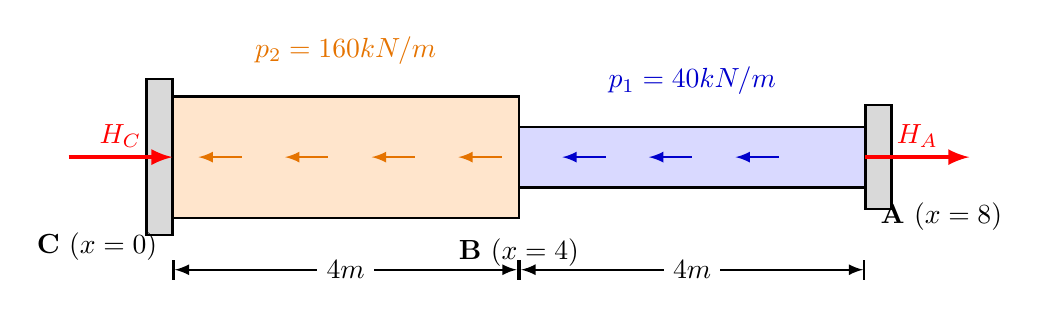
\begin{tikzpicture}[scale=1.1, >=latex]
        % Barra horizontal C -> B -> A
        \draw[thick, fill=orange!20] (0,-0.7) rectangle (4,0.7);
        \draw[thick, fill=blue!15] (4,-0.35) rectangle (8,0.35);
        
        % Apoyos
        \draw[thick, fill=gray!30] (-0.3,-0.9) rectangle (0,0.9);
        \draw[thick, fill=gray!30] (8,-0.6) rectangle (8.3,0.6);
        
        % Reacciones
        \draw[ultra thick, red, ->] (-1.2,0) -- (0,0);
        \node[red, above] at (-0.6,0) {$H_C$};
        \draw[ultra thick, red, ->] (8,0) -- (9.2,0);
        \node[red, above] at (8.6,0) {$H_A$};
        
        % Flechas de carga distribuida (peso hacia C, es decir, hacia la izquierda)
        \foreach \i in {0.8, 1.8, 2.8, 3.8} {
            \draw[thick, orange!90!black, <-] (\i-0.5,0) -- (\i,0);
        }
        \node[orange!90!black, above=8pt] at (2,0.7) {$p_2 = 160\text{ kN/m}$};
        
        \foreach \i in {5.0, 6.0, 7.0} {
            \draw[thick, blue!80!black, <-] (\i-0.5,0) -- (\i,0);
        }
        \node[blue!80!black, above=8pt] at (6,0.35) {$p_1 = 40\text{ kN/m}$};
        
        % Cotas y nudos
        \node[below left=2pt] at (0,-0.7) {$\mathbf{C}$ ($x = 0$)};
        \node[below=4pt] at (4,-0.7) {$\mathbf{B}$ ($x = 4$)};
        \node[below right=2pt] at (8,-0.35) {$\mathbf{A}$ ($x = 8$)};
        
        \draw[|<->|, thick] (0,-1.3) -- (4,-1.3) node[midway, fill=white] {$4\text{ m}$};
        \draw[|<->|, thick] (4,-1.3) -- (8,-1.3) node[midway, fill=white] {$4\text{ m}$};
    \end{tikzpicture}
    \caption{Modelo equivalente horizontal con origen de coordenadas en el apoyo inferior $C$.}
    \label{fig:barra_horizontal_dcl}
\end{figure}

Planteando el equilibrio de fuerzas axiles horizontales:
\begin{equation}
    \sum F_x = 0 \implies H_A + H_C - P_{\text{total}} = 0 \implies H_A + H_C = 800\text{ kN} \label{eq:escalonada_equilibrio}
\end{equation}
El problema presenta 1 grado de hiperestatismo (2 incógnitas de reacción para 1 ecuación de equilibrio axial no trivial).

\subsection{Ecuación de Compatibilidad de Deformaciones}

Los apoyos rígidos en $A$ y $C$ impiden el desplazamiento relativo total entre ambos extremos:
\begin{equation}
    \Delta L_{AC} = \Delta L_{BC} + \Delta L_{AB} = 0 \label{eq:escalonada_compatibilidad}
\end{equation}
Expresando el alargamiento elástico en función de la ley del esfuerzo axil $N(x)$:
\begin{equation}
    \Delta L_{AC} = \int_{0}^{4} \frac{N(x)}{\Omega_2 E}\,dx + \int_{4}^{8} \frac{N(x)}{\Omega_1 E}\,dx = 0
\end{equation}
Al ser el módulo elástico $E$ constante en toda la barra, se simplifica directamente:
\begin{equation}
    \frac{1}{\Omega_2} \int_{0}^{4} N(x)\,dx + \frac{1}{\Omega_1} \int_{4}^{8} N(x)\,dx = 0 \implies \frac{1}{8} \int_{0}^{4} N(x)\,dx + \frac{1}{2} \int_{4}^{8} N(x)\,dx = 0 \label{eq:escalonada_integral}
\end{equation}

\begin{tcolorbox}[colback=blue!5!white, colframe=blue!60!black, arc=3pt, boxrule=0.7pt]
    \small \textbf{Consejo Metodológico Clave (Anotación del Examen):}
    Si planteamos los cortes por secciones siempre mirando hacia la izquierda (desde el apoyo $C$, $x = 0$), en la ley de axiles $N(x)$ de ambos tramos solo intervendrá la reacción $H_C$. De esta forma, la ecuación de compatibilidad se resuelve con una única incógnita directa, evitando resolver sistemas de ecuaciones simultáneos acoplados.
\end{tcolorbox}

\subsubsection{Leyes del Esfuerzo Axil por Tramos}

\begin{enumerate}
    \item \textbf{Tramo 1: $BC$ ($x \in [0, 4\text{ m}]$, sección $\Omega_2 = 8\text{ m}^2$)}:
    Cortando a una distancia $x$ desde $C$ y aislando la parte izquierda:
    \begin{equation}
        \sum F_x = 0 \implies H_C - p_2 \cdot x + N(x) = 0
    \end{equation}
    \begin{equation}
        N(x) = 160\,x - H_C \label{eq:axil_tramo1}
    \end{equation}

    \item \textbf{Tramo 2: $AB$ ($x \in [4, 8\text{ m}]$, sección $\Omega_1 = 2\text{ m}^2$)}:
    Cortando en el tramo $AB$ a una distancia $x$ desde $C$ (abarcando todo el tramo $BC$ de $4\text{ m}$ y una longitud $x - 4$ del tramo $AB$):
    \begin{equation}
        \sum F_x = 0 \implies H_C - 160(4) - 40(x - 4) + N(x) = 0
    \end{equation}
    \begin{equation}
        N(x) = H_C - 640 - 40x + 160 + N(x) = 0 \implies N(x) = 40\,x - H_C + 480 \label{eq:axil_tramo2}
    \end{equation}
\end{enumerate}

\subsection{Resolución de las Reacciones en los Apoyos}

Sustituyendo las leyes de esfuerzos~\eqref{eq:axil_tramo1} y \eqref{eq:axil_tramo2} en la ecuación de compatibilidad~\eqref{eq:escalonada_integral}:
\begin{equation}
    \frac{1}{8} \int_{0}^{4} (160\,x - H_C)\,dx + \frac{1}{2} \int_{4}^{8} (40\,x - H_C + 480)\,dx = 0
\end{equation}

Calculando cada integral elemental:
\begin{align}
    \int_{0}^{4} (160\,x - H_C)\,dx &= \left[ 80\,x^2 - H_C\,x \right]_0^4 = 80(16) - 4\,H_C = 1280 - 4\,H_C \\[6pt]
    \int_{4}^{8} (40\,x - H_C + 480)\,dx &= \left[ 20\,x^2 + (480 - H_C)x \right]_4^8 \nonumber \\
    &= \left[ 20(64) + 8(480 - H_C) \right] - \left[ 20(16) + 4(480 - H_C) \right] \nonumber \\
    &= \left[ 1280 + 3840 - 8\,H_C \right] - \left[ 320 + 1920 - 4\,H_C \right] \nonumber \\
    &= (5120 - 8\,H_C) - (2240 - 4\,H_C) = 2880 - 4\,H_C
\end{align}

Sustituyendo en la expresión con los factores de sección:
\begin{align}
    \frac{1}{8}(1280 - 4\,H_C) + \frac{1}{2}(2880 - 4\,H_C) &= 0 \nonumber \\
    \left(160 - \frac{H_C}{2}\right) + (1440 - 2\,H_C) &= 0 \nonumber \\
    1600 - 2{,}5\,H_C &= 0 \implies \mathbf{H_C = \frac{1600}{2{,}5} = 640\text{ kN}}
\end{align}

A partir de la ecuación de equilibrio estático global~\eqref{eq:escalonada_equilibrio}:
\begin{equation}
    H_A = 800\text{ kN} - H_C = 800 - 640 \implies \mathbf{H_A = 160\text{ kN}}
\end{equation}

\begin{tcolorbox}[colback=myg!10!white, colframe=myg!70!black, arc=3pt, boxrule=0.8pt]
    \textbf{Interpretación Física de las Reacciones:}
    \begin{itemize}
        \item Apoyo inferior $C$: Soporta $H_C = 640\text{ kN}$ a compresión, absorbiendo exactamente el peso de su propio tramo $BC$ ($640\text{ kN}$).
        \item Apoyo superior $A$: Retiene $H_A = 160\text{ kN}$ a tracción, soportando en suspensión el peso completo de su tramo $AB$ ($160\text{ kN}$).
        \item El nudo de transición $B$ resulta ser una sección de \textbf{esfuerzo axil estrictamente nulo} ($N(4) = 0$).
    \end{itemize}
\end{tcolorbox}

\subsection{Leyes Numéricas y Diagramas de Esfuerzos Axiles y Tensiones}

Sustituyendo el valor $H_C = 640\text{ kN}$ en las leyes analíticas:

\subsubsection{1. Ley del Esfuerzo Axil}
\begin{itemize}
    \item \textbf{Tramo $BC$ ($x \in [0, 4\text{ m}]$):}
    \begin{align}
        N(x) &= 160\,x - 640\text{ kN} \\
        x &= 0 \implies N_C = -640\text{ kN} \quad (\text{Compresión}) \\
        x &= 4 \implies N_B = 160(4) - 640 = \mathbf{0\text{ kN}}
    \end{align}
    \item \textbf{Tramo $AB$ ($x \in [4, 8\text{ m}]$):}
    \begin{align}
        N(x) &= 40\,x - 640 + 480 = 40\,x - 160\text{ kN} \\
        x &= 4 \implies N_B = 40(4) - 160 = \mathbf{0\text{ kN}} \\
        x &= 8 \implies N_A = 40(8) - 160 = \mathbf{+160\text{ kN}} \quad (\text{Tracción})
    \end{align}
\end{itemize}

\subsubsection{2. Ley de Tensiones Normales}
\begin{itemize}
    \item \textbf{Tramo $BC$ ($\Omega_2 = 8\text{ m}^2$):}
    \begin{align}
        \sigma(x) &= \frac{160\,x - 640}{8} = 20\,x - 80\text{ kN/m}^2 \\
        x &= 0 \implies \sigma_C = -80\text{ kN/m}^2 = -80\text{ kPa} \quad (\text{Compresión máxima}) \\
        x &= 4 \implies \sigma_B = 0\text{ kN/m}^2
    \end{align}
    \item \textbf{Tramo $AB$ ($\Omega_1 = 2\text{ m}^2$):}
    \begin{align}
        \sigma(x) &= \frac{40\,x - 160}{2} = 20\,x - 80\text{ kN/m}^2 \\
        x &= 4 \implies \sigma_B = 0\text{ kN/m}^2 \\
        x &= 8 \implies \sigma_A = +80\text{ kN/m}^2 = +80\text{ kPa} \quad (\text{Tracción máxima})
    \end{align}
\end{itemize}

\begin{tcolorbox}[colback=orange!10!white, colframe=orange!85!black, arc=3pt, boxrule=0.7pt]
    \small \textbf{Particularidad Singular del Diagrama de Tensiones:}
    Aunque la ley del esfuerzo axil $N(x)$ cambia de pendiente al pasar del tramo 1 al tramo 2 ($160\text{ kN/m} \to 40\text{ kN/m}$), la ley de tensiones normales $\sigma(x) = \frac{N(x)}{\Omega(x)}$ tiene \textbf{la misma pendiente en ambos tramos} ($\frac{160}{8} = \frac{40}{2} = \gamma = 20\text{ kN/m}^3$) y es completamente continua en toda la longitud de la barra, variando linealmente desde $-80\text{ kPa}$ hasta $+80\text{ kPa}$.
\end{tcolorbox}

\begin{figure}[H]
    \centering
    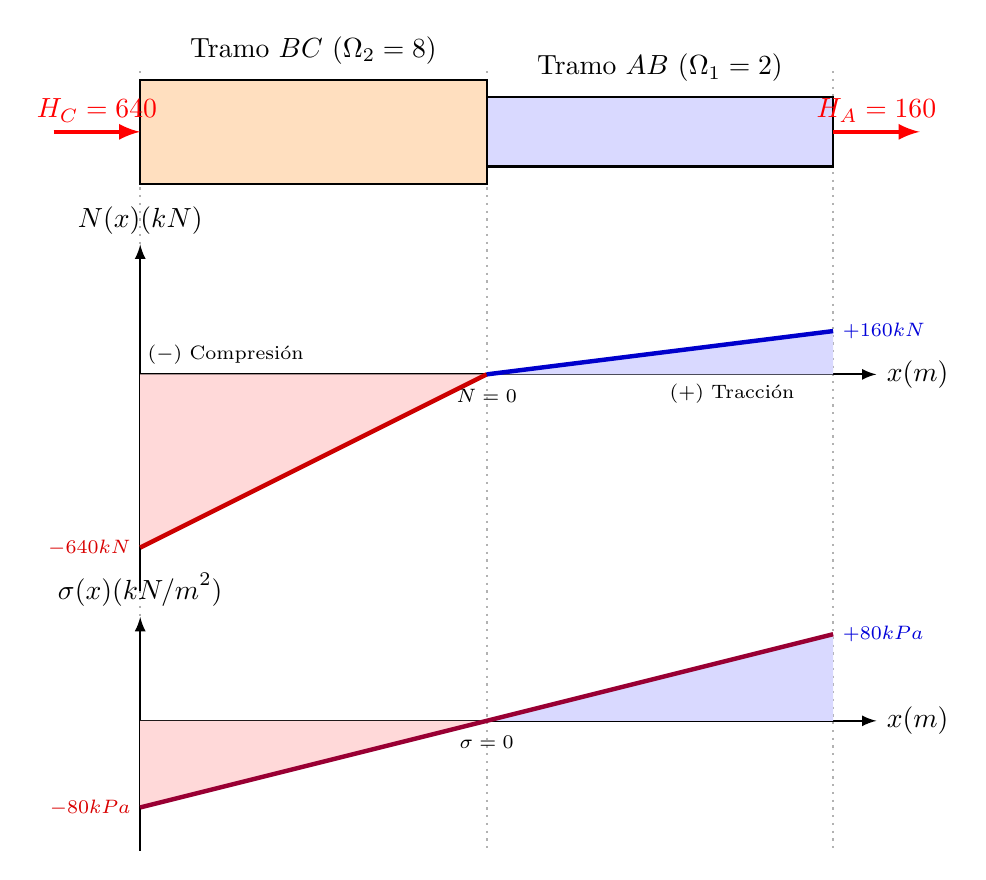
\begin{tikzpicture}[scale=1.1, >=latex]
        % Eje de referencia horizontal
        \draw[dotted, thick, gray!60] (0,2.5) -- (0,-6.5);
        \draw[dotted, thick, gray!60] (4,2.5) -- (4,-6.5);
        \draw[dotted, thick, gray!60] (8,2.5) -- (8,-6.5);
        
        % ESQUEMA MECÁNICO
        \draw[thick, fill=orange!25] (0,1.2) rectangle (4,2.4);
        \draw[thick, fill=blue!15] (4,1.4) rectangle (8,2.2);
        \node[above=2pt] at (2,2.4) {Tramo $BC$ ($\Omega_2 = 8$)};
        \node[above=2pt] at (6,2.2) {Tramo $AB$ ($\Omega_1 = 2$)};
        
        \draw[ultra thick, red, ->] (-1.0,1.8) -- (0,1.8);
        \node[red, above] at (-0.5,1.8) {$H_C = 640$};
        \draw[ultra thick, red, ->] (8,1.8) -- (9.0,1.8);
        \node[red, above] at (8.5,1.8) {$H_A = 160$};
        
        % DIAGRAMA DE ESFUERZOS AXILES N(x)
        \draw[thick, ->] (0,-1.0) -- (8.5,-1.0) node[right] {$x\text{ (m)}$};
        \draw[thick, ->] (0,-3.5) -- (0,0.5) node[above] {$N(x)\text{ (kN)}$};
        
        % Linea base en y = -1.0
        % N(0) = -640 -> y = -1.0 - 2.0 = -3.0
        % N(4) = 0    -> y = -1.0
        % N(8) = +160 -> y = -1.0 + 0.8 = -0.2
        \fill[red!15] (0,-1.0) -- (0,-3.0) -- (4,-1.0) -- cycle;
        \draw[ultra thick, red!80!black] (0,-3.0) -- (4,-1.0);
        
        \fill[blue!15] (4,-1.0) -- (8,-0.5) -- (8,-1.0) -- cycle;
        \draw[ultra thick, blue!80!black] (4,-1.0) -- (8,-0.5);
        
        \node[left, font=\bfseries\scriptsize, red!85!black] at (0,-3.0) {$-640\text{ kN}$};
        \node[right, font=\bfseries\scriptsize, blue!85!black] at (8,-0.5) {$+160\text{ kN}$};
        \node[below=2pt, font=\bfseries\scriptsize] at (4,-1.0) {$N=0$};
        \node[above left, font=\scriptsize] at (2,-1.0) {$(-)$ Compresión};
        \node[below right, font=\scriptsize] at (6,-1.0) {$(+)$ Tracción};
        
        % DIAGRAMA DE TENSIONES NORMALES sigma(x)
        \draw[thick, ->] (0,-5.0) -- (8.5,-5.0) node[right] {$x\text{ (m)}$};
        \draw[thick, ->] (0,-6.5) -- (0,-3.8) node[above] {$\sigma(x)\text{ (kN/m}^2)$};
        
        % Linea continua de -80 a +80
        % sigma(0) = -80 -> y = -5.0 - 1.0 = -6.0
        % sigma(4) = 0   -> y = -5.0
        % sigma(8) = +80 -> y = -5.0 + 1.0 = -4.0
        \fill[red!15] (0,-5.0) -- (0,-6.0) -- (4,-5.0) -- cycle;
        \fill[blue!15] (4,-5.0) -- (8,-4.0) -- (8,-5.0) -- cycle;
        \draw[ultra thick, purple!80!black] (0,-6.0) -- (8,-4.0);
        
        \node[left, font=\bfseries\scriptsize, red!85!black] at (0,-6.0) {$-80\text{ kPa}$};
        \node[right, font=\bfseries\scriptsize, blue!85!black] at (8,-4.0) {$+80\text{ kPa}$};
        \node[below=2pt, font=\bfseries\scriptsize] at (4,-5.0) {$\sigma=0$};
    \end{tikzpicture}
    \caption{Diagramas analíticos de esfuerzo axil $N(x)$ y tensión normal $\sigma(x)$.}
    \label{fig:diagramas_barra_escalonada}
\end{figure}

%=============================================================================
\subsection*{Resumen Final de Resultados}

\begin{table}[H]
    \centering
    \caption{Resumen analítico y numérico del problema de barra escalonada biapoyada.}
    \vspace{2mm}
    \adjustbox{max width=0.92\textwidth}{%
        \renewcommand{\arraystretch}{1.3}
        \begin{tabular}{lccc}
            \toprule
            \textbf{Magnitud} & \textbf{Símbolo / Expresión} & \textbf{Valor Numérico} & \textbf{Estado Físico} \\
            \midrule
            Reacción en apoyo inferior $C$ & $H_C$ & $\mathbf{640{,}00\text{ kN}}$ & Compresión ($\uparrow$) \\
            Reacción en apoyo superior $A$ & $H_A$ & $\mathbf{160{,}00\text{ kN}}$ & Tracción ($\uparrow$) \\
            \midrule
            Esfuerzo axil en $C$ ($x = 0$) & $N_C$ & $\mathbf{-640{,}00\text{ kN}}$ & Compresión máxima \\
            Esfuerzo axil en cambio sección $B$ & $N_B$ & $\mathbf{0{,}00\text{ kN}}$ & Punto neutro \\
            Esfuerzo axil en $A$ ($x = 8\text{ m}$) & $N_A$ & $\mathbf{+160{,}00\text{ kN}}$ & Tracción máxima \\
            \midrule
            Tensión normal en $C$ & $\sigma_C = N_C/\Omega_{BC}$ & $\mathbf{-80{,}00\text{ kPa}}$ & Compresión máxima \\
            Tensión normal en $A$ & $\sigma_A = N_A/\Omega_{AB}$ & $\mathbf{+80{,}00\text{ kPa}}$ & Tracción máxima \\
            \bottomrule
        \end{tabular}%
    }
    \label{tab:resumen_barra_escalonada}
\end{table}

%=============================================================================
